\documentclass[a4paper, 10pt, garamond]{book}
\usepackage{cours-preambule}
\usepackage{tocloft}

\renewcommand{\mtcSfont}{\Large}
\setlength{\mtcindent}{5pt}
\mtcsetoffset{minitoc}{-5pt}
\addtolength{\cftsecnumwidth}{10pt}
\setcounter{minitocdepth}{1}

\dominitoc
\faketableofcontents

% \toggletrue{student}
% \HideSolutionstrue
% \toggletrue{corrige}
% \renewcommand{\mycol}{black}
\renewcommand{\mycol}{gray}

\makeatletter
\renewcommand{\@chapapp}{MPSI3 -- 24 novembre 2023 -- Devoir surveillé}
\makeatother

\graphicspath{{./figures/}{./figures/E1}{./figures/E2}{./figures/P1}{./figures/P2}}

\newcommand{\figsvg}[1]{
  \begin{center}
    \subimport{figures/}{#1}
  \end{center}
}
\newcommand{\figsvgCap}[2]{
  \begin{center}
    \subimport{figures/}{#1}
    \captionof{figure}{#2}
  \end{center}
}

\setlist[blocQR,1]{leftmargin=10pt, label=\sqenumi}
\counterwithin*{equation}{section}

\begin{document}
\setcounter{chapter}{2}
\chapter{\cswitch{Correction du DS}{Oscillateurs et transformation de la
	  matière}}
\label{ch:ds03}

\enonce{
	\begin{center}
		\Large\bfseries
		Tout moyen de communication est interdit
		\smallbreak
		Les téléphones portables doivent être éteints et rangés dans les sacs
		\smallbreak
		\xul{Les calculatrices sont \textit{autorisées}}
	\end{center}
	\begin{tcb}*[cnt, bld](ror)<itc>{Au programme}
		\large
		Oscillateurs harmonique et amortis (mécanique et électricité),
		transformation et équilibre chimique.
	\end{tcb}
	\vfill
	\minitoc
	\vfill

	Les différentes questions peuvent être traitées dans l'ordre désiré.
	\textbf{Cependant}, vous indiquerez le numéro correct de chaque question. Vous
	prendrez soin d'indiquer sur votre copie si vous reprenez une question d'un
	exercice plus loin dans la copie, sous peine qu'elle ne soit ni vue ni corrigée.
	\bigbreak
	Vous porterez une attention particulière à la \textbf{qualité de rédaction}.
	Vous énoncerez clairement les hypothèses, les lois et théorèmes utilisés. Les
	relations mathématiques doivent être reliées par des connecteurs logiques.
	\bigbreak
	Vous prendre soin de la \textbf{présentation} de votre copie, notamment au
	niveau de l'écriture, de l'orthographe, des encadrements, de la marge et du
	cadre laissé pour la note et le commentaire. Vous \textbf{encadrerez les
		expressions littérales}, sans faire apparaître les calculs. Vous ferez
	apparaître cependant le détail des grandeurs avec leurs unités. Vous
	\textbf{soulignerez les applications numériques}.
	\bigbreak
	Ainsi, l'étudiant-e s'expose aux malus suivants concernant la forme et le fond~:
	\begin{tcb}*(prop)"bomb"{Malus}
		\begin{minipage}[t]{0.50\linewidth}
			\begin{itemize}
				\item A~: application numérique mal faite~;
				\item N~: numéro de copie manquant~;
				\item P~: prénom manquant~;
				\item E~: manque d'encadrement des réponses~;
				\item M~: marge non laissée ou trop grande~;
				\item V~: confusion ou oubli de vecteurs~;
			\end{itemize}
		\end{minipage}
		\begin{minipage}[t]{0.50\linewidth}
			\begin{itemize}
				\item Q~: question mal ou non indiquée~;
				\item C~: copie grand carreaux~;
				\item U~: mauvaise unité (flagrante)~;
				\item H~: homogénéité non respectée~;
				\item S~: chiffres significatifs non cohérents~;
				\item $\f$~: loi physique fondamentale brisée.
			\end{itemize}
		\end{minipage}
	\end{tcb}

	% \begin{tcb}(impo){Exemple application numérique}
	% 	\vspace*{-10pt}
	% 	\begin{minipage}[c]{0.45\linewidth}
	% 		\begin{gather*}
	% 			\boxed{n = \frac{PV}{RT}}
	% 			\qav
	% 			\left\{
	% 			\begin{array}{rcl}
	% 				p & = & \SI{1.0e5}{Pa}                \\
	% 				V & = & \SI{1.0e-3}{m^3}              \\
	% 				R & = & \SI{8.314}{J.mol^{-1}.K^{-1}} \\
	% 				T & = & \SI{300}{K}
	% 			\end{array}
	% 			\right.\\
	% 			\mathrm{A.N.~:}\quad
	% 			\xul{n = \SI{5.6e-4}{mol}}
	% 		\end{gather*}
	% 	\end{minipage}
	% 	\hfill
	% 	\cancel{\bcancel{
	% 			\begin{minipage}[c]{0.45\linewidth}
	% 				\begin{gather*}
	% 					n = \frac{PV}{RT} = \frac{\num{e5}\cdot\num{1}}{8.32\cdot300}
	% 					= 0.56
	% 				\end{gather*}
	% 			\end{minipage}
	% 		}}
	% \end{tcb}
	\vfill
	\newpage
}

\setcounter{section}{0}
\exercice[23]{Pentachlorure de phosphore}
\resetQ
\enonce{
Le pentachlorure de phosphore \ce{PCl5} est un composé très toxique, servant
de réactif en synthèse organique pour ajouter des atomes de chlore à une
chaîne carbonée. Mis en phase gazeuse, il se décompose spontanément en
trichlorure de phosphore et en dichlore, donnant naissance à un équilibre en
phase gazeuse.

Considérons un réacteur fermé de volume constant $V = \SI{2}{L}$ maintenu à
température constante $T = \SI{180}{\celsius}$. À cette température, la
constante thermodynamique de l’équilibre précédemment cité vaut $K^\circ =
	8$. On y met $n_0 = \SI{0,5}{\mol}$ de \ce{PCl5}.

On rappelle que $R = \SI{8.314}{J.K^{-1}.mol^{-1}}$.
}

\QR[3]{%
	Exprimer puis calculer la pression initiale dans le réacteur $p_0$ en fonction
	des données.
}{%
	On applique la loi des gaz parfaits~:
	\begin{gather*}
		\boxed{p_0=\frac{n_0RT}{V}}
		\qav
		\left\{
		\begin{array}{rcl}
			n_0 & = & \SI{0.5}{mol}
			\\
			R   & = & \SI{8.314}{J.K^{-1}.mol^{-1}}
			\\
			T   & = & \SI{453.15}{K}
			\\
			V   & = & \SI{2e-3}{m^{3}}
		\end{array}
		\right.\\
		\AN
		\xul{
			p_0 = \SI{9.41e5}{Pa}
		}
	\end{gather*}
}

\QR[5]{%
	Écrire l’équation de réaction modélisant le processus dans le réacteur, et
	dresser le tableau d'avancement correspondant.
}{%
	\begin{center}
		\def\rhgt{0.35}
		\centering
		\begin{tabularx}{.7\linewidth}{|l|c||YdYdY||Y|}
			\hline
			\multicolumn{2}{|c||}{%
				$\xmathstrut{\rhgt}$
			\textbf{Équation}}  &
			$\ce{PCl_5\gaz{}}$  & $=$                   &
			$\ce{PCl_3\gaz{}}$  & $+$                   &
			$\ce{Cl_2\gaz{}}$   &
			$n_{\tot, gaz}$                               \\
			\hline
			$\xmathstrut{\rhgt}$
			Initial             & $\xi = 0$             &
			$n_0$               & \vline                &
			$0$                 & \vline                &
			$0$                 &
			$n_0$                                         \\
			\hline
			$\xmathstrut{\rhgt}$
			Interm.             & $\xi$                 &
			$n_0 - \xi$         & \vline                &
			$\xi$               & \vline                &
			$\xi$               &
			$n_0 + \xi$                                   \\
			\hline
			$\xmathstrut{\rhgt}$
			Final               & $\xi_f = \xi\ind{eq}$ &
			$n_0 - \xi\ind{eq}$ & \vline                &
			$\xi\ind{eq}$       & \vline                &
			$\xi\ind{eq}$       &
			$n_0 + \xi\ind{eq}$                           \\
			\hline
		\end{tabularx}
	\end{center}
}

\QR[3]{%
	Exprimer les pressions partielles des gaz en fonction de $n_0$, $\xi$ et de la
	pression initiale $p_0$.
}{%
	On utilise à nouveau l'équation des gaz parfaits, avec $\frac{RT}{V} =
		\frac{p_0}{n_0}$~:
	\[
		\boxed{P_{\ce{PCl5}} = \frac{(n_0-\xi)RT}{V}=\frac{(n_0-\xi)p_0}{n_0}}
		\qqet
		\boxed{P_{\ce{PCl3}} = \frac{\xi p_0}{n_0}}
		\qqet
		\boxed{P_{\ce{Cl2}} = \frac{\xi p_0}{n_0}}
	\]
}

\QR[9]{%
	Exprimer le coefficient de dissociation à l’équilibre $\alpha = \xi\ind{eq}
		/n_0$ en fonction de $K^\circ $, $p^\circ $ et $p_0$. Faire l'application
	numérique. Que représente-t-il physiquement~?
}{%
	\noindent
	\begin{minipage}[t]{.5\linewidth}
		Loi d'action de masses~:
		\begin{DispWithArrows*}[fleqn, mathindent=10pt]
			K^\circ &=
			\eval{\frac{a(\ce{PCl3})a(\ce{Cl2})}{a(\ce{PCl5})}}\ind{eq}
			\Arrow{Activité d'un gaz}
			\\\Lra
			K^\circ &=
			\eval{
				\frac{\frac{P_{\ce{PCl3}}}{p^\circ}\frac{P_{\ce{Cl2}}}{p^\circ}}
				{\frac{P_{\ce{PCl5}}}{p^\circ}}}\ind{eq}
			\Arrow{Question 2}
			\\\Lra
			K^\circ &=
			\frac{\xi\ind{eq}^2}{n_0(n_0-\xi\ind{eq})}\frac{p_0}{p^\circ}
			\Arrow{On factorise}
			\\\Lra
			K^\circ &=
			\underbracket[1pt]{\cancel{\frac{n_0^{2}}{n_0^{2}}}}_{=1}
			\frac{\left( \frac{\xi\ind{eq}}{n_0} \right)^{2}}{1 \left(
				1-\frac{\xi\ind{eq}}{n_0} \right)}
			\frac{p_0}{p^\circ}
			\Arrow{$\alpha = \xi\ind{eq}/n_0$}
			\\\Lra
			K^\circ &=
			\frac{\alpha^2}{(1-\alpha)}\frac{p_0}{p^\circ }
		\end{DispWithArrows*}
	\end{minipage}
	\hfill
	\begin{minipage}[t]{.5\linewidth}
		Ainsi, en isolant~:
		\begin{DispWithArrows*}
			\alpha^2 &+ \alpha\left(\frac{K^\circ p^\circ }{p_0} \right) -
			\frac{K^\circ p^\circ }{p_0} = 0
			% \Arrow{$\Delta$ son discriminant}
			\\\Ra
			\Delta &=
			\left(\frac{K^\circ p^\circ }{p_0} \right)^2 +
			4\left(\frac{K^\circ p^\circ }{p_0} \right) > 0
			% \Arrow{Solution positive}
			\\\Lra
			\Aboxed{
				\alpha &= -\left(\frac{K^\circ p^\circ }{2p_0} \right) +
				\sqrt{\left(\frac{K^\circ p^\circ }{2p_0} \right)^2 +
					\left(\frac{K^\circ p^\circ }{p_0} \right)}}
			\\\Ra
			\makebox[0pt][l]{$\phantom{\AN}\xul{\phantom{\alpha = \num{0.59}}}$}
			\AN
			\alpha &= \num{0.59}
		\end{DispWithArrows*}
		$\alpha$ représente la proportion de réactif ayant effectivement réagit.
	\end{minipage}
}

\QR[3]{%
	Exprimer la pression à l'équilibre en fonction $p_0$ et $\alpha$. La calculer.
}{%
	À l'aide du tableau d'avancement, on a $n\ind{tot, gaz}$, d'où

	\begin{gather*}
		P\ind{eq} = \frac{n_0+\xi\ind{eq}}{n_0}p_0
		\Lra
		\boxed{
			P\ind{eq} = (1+\alpha)p_0
		}
		\\
		\AN
		\xul{P\ind{eq} = \SI{15,0}{bar}}
	\end{gather*}
}

\iftoggle{corrige}{}{%
	\newpage
}

\resetQ
\exercice[41]{États finaux variés}
\enonce{
	On s'intéresse dans un premier temps à une solution aqueuse obtenue à
	\SI{298}{K} par un mélange d'acide éthanoïque \ce{CH3COOH} (concentration
	$c_1=\SI{0.10}{mol.L^{-1}}$ après mélange) et d'ions fluorure \ce{F-}
	(concentration $c_2=\SI{5.0e-2}{mol.L^{-1}}$ après mélange).
	La réaction \eqref{eq:R1} susceptible de se produire s'écrit~:
	\begin{alignat}{2}
		\ce{CH3COOH(aq) + F^-(aq) & = CH3COO^-(aq) & + HF(aq)}
		\tag{1}\label{eq:R1}
		\\
		\intertext{On connaît les constantes d'équilibre à \SI{298}{K} des réactions
			suivantes~:}
		\beforetext{$K^\circ_2 = \num{e-4.8}$}
		\ce{CH3COOH(aq) + H2O     & = CH3COO^-(aq) & + H3O^+(aq)}
		\tag{2}\label{eq:R2}
		\\
		\beforetext{$K^\circ_3 = \num{e-3.2}$}
		\ce{HF(aq) + H2O          & = F^-(aq)      & + H3O^+(aq)}
		\tag{3}\label{eq:R3}
	\end{alignat}
}

\QR[3]{%
	Exprimer la constante $K_1^\circ$ relative à l'équilibre~\eqref{eq:R1} en
	fonction d'autres constantes de réaction, puis la calculer. Donner le résultat
	sous la forme d'une puissance de 10 uniquement.
}{%
	On constate que l'équilibre%
	\sswitch{%
		$(1) = (2) - (3)$
	}{%
		$\eqref{eq:R1}=\eqref{eq:R2}-\eqref{eq:R3}$
	}%
	donc
	\[
		\boxed{K^\circ_1=\cfrac{K^\circ_2}{K^\circ_3}=\num{e-1.6}}
	\]
}

\QR[10]{%
	Déterminer l'état d'équilibre de la solution issue du mélange de l'acide
	éthanoïque et des ions fluorure~: exprimer l'équation dont l'avancement est
	solution, et l'expression littérale de la solution en fonction de $c_1$, $c_2$
	et $K_1^\circ$.
}{%
	On dresse le tableau d'avancement en concentration~:
	\begin{center}
		\def\rhgt{0.35}
		\centering
		\begin{tabularx}{\linewidth}{|l|c||YdYdYdY|}
			\hline
			\multicolumn{2}{|c||}{%
				$\xmathstrut{\rhgt}$
			\textbf{Équation}}        &
			$\ce{CH_3COOH(aq)}$       & $+$               &
			$\ce{F^{-}(aq)}$          & $\ra$             &
			$\ce{CH_3COO^{-}(aq)}$    & $+$               &
			$\ce{HF(aq)}$                                   \\
			\hline
			$\xmathstrut{\rhgt}$
			Initial                   & $x = 0$           &
			$c_1$                     & \vline            &
			$c_2$                     & \vline            &
			$0$                       & \vline            &
			$0$                                             \\
			\hline
			$\xmathstrut{\rhgt}$
			Interm.                   & $x$               &
			$c_1 - x$                 & \vline            &
			$c_2 - x$                 & \vline            &
			$x$                       & \vline            &
			$x$                                             \\
			\hline
			$\xmathstrut{\rhgt}$
			Final ($\si{mol.L^{-1}}$) & $x_f = x\ind{eq}$ &
			$\num{9.0e-2}$            & \vline            &
			$\num{4.0e-2}$            & \vline            &
			$\num{9.6e-3}$            & \vline            &
			$\num{9.6e-3}$                                  \\
			\hline
		\end{tabularx}
	\end{center}

	D'après la loi d'action de masse,
	\begin{DispWithArrows*}[groups]
		K^\circ_1 &= \cfrac{x\ind{eq}^2}{(c_1-x\ind{eq})\times (c_2-x\ind{eq})}
		\Arrow{On isole}
		\\\Lra
		(c_1-x\ind{eq})(c_2-x\ind{eq})K^\circ_1 &= x\ind{eq}^{2}
		\Arrow[new-group]{On rassemble}
		\\\Lra
		x\ind{eq}^{2} + (x\ind{eq}-c_1)(x\ind{eq}-c_2)K^\circ_1 &= 0
		\Arrow{On développe et factorise}
		\\\Lra
		\Aboxed{
			x\ind{eq}^{2}(1+K^\circ_1) -
			x\ind{eq}(c_1+c_2)K^\circ_1 + c_1c_2K^\circ_1 &= 0
		}
	\end{DispWithArrows*}
	Ainsi, avec $\Delta$ le discriminant de ce trinôme~:
	\begin{DispWithArrows*}
		\Delta &= \left( c_1+c_2 \right)^{2}\left( K_1^\circ \right)^{2}
		-4(1+K_1^\circ)c_1c_2K_1^\circ
		\Arrow{Solutions}
		\\\Ra
		\Aboxed{
			x_{\equ,\pm} &=
			\frac{
				(c_1+c_2)K_1^\circ \pm \sqrt{
					\left( c_1+c_2 \right)^{2}\left( K_1^\circ \right)^{2}
					-4(1+K_1^\circ)c_1c_2K_1^\circ}
			}{2(1+K_1^\circ)}
		}
		\Arrow{Calcul}
		\\
		\makebox[0pt][l]{%
			$\phantom{\AN}\xul{\phantom{x\ind{eq} = \SI{9.6e-3}{mol.L^{-1}}}}$%
		}
		\AN
		x\ind{eq} &= \SI{9.6e-3}{mol.L^{-1}}
		\qav
		\left\{
		\begin{array}{rcl}
			c_1       & = & \SI{0.1}{mol.L^{-1}}
			\\
			c_2       & = & \SI{5.0e-2}{mol.L^{-1}}
			\\
			K_1^\circ & = & \num{e-1.6}
		\end{array}
		\right.
	\end{DispWithArrows*}
	On en déduit les concentrations à l'équilibre indiquées dans le tableau.
}

\enonce{
	On étudie dans la suite de l'exercice quelques constituants du béton.
	L'hydroxyde de calcium \ce{Ca(OH)_2(s)} confère au béton ses propriétés
	basiques (au sens de acide ou base). Il se dissout en solution aqueuse selon
	la réaction~\eqref{eq:R4}~:
	\begin{gather}
		\beforetext{$K^\circ_4(\SI{298}{K}) = \num{e-5.2}$}
		\ce{Ca(OH)_2(s) = Ca^{2+}(aq) + 2HO^-(aq)}
		\tag{4}\label{eq:R4}
	\end{gather}
}

\QR[6]{%
	On introduit en solution aqueuse un net excès d'hydroxyde de calcium. La phase
	solide est alors présente en fin d'évolution. Calculer les concentrations de
	chacun des ions présents à l'équilibre.
}{%
	On dresse un tableau d'avancement en concentration~:
	\begin{center}
		\def\rhgt{0.35}
		\centering
		\begin{tabularx}{.7\linewidth}{|l|c||YdYdY|}
			\hline
			\multicolumn{2}{|c||}{%
				$\xmathstrut{\rhgt}$
			\textbf{Équation}}        &
			$\ce{Ca(OH)2(s)}$         & $=$               &
			$\ce{Ca^{2+}(aq)}$        & $+$               &
			$2\ce{HO^{-}(aq)}$                              \\
			\hline
			$\xmathstrut{\rhgt}$
			Initial                   & $x = 0$           &
			excès                     & \vline            &
			$0$                       & \vline            &
			$0$                                             \\
			\hline
			$\xmathstrut{\rhgt}$
			Interm.                   & $x$               &
			excès                     & \vline            &
			$x$                       & \vline            &
			$2x$                                            \\
			\hline
			$\xmathstrut{\rhgt}$
			Final ($\si{mol.L^{-1}}$) & $x_f = x\ind{eq}$ &
			excès                     & \vline            &
			$\num{1.2e-2}$            & \vline            &
			$\num{2.4e-2}$                                  \\
			\hline
		\end{tabularx}
	\end{center}
	\begin{gather*}
		\beforetext{Par la loi d'action de masse,}
		K^\circ_4=x\ind{eq}\times (2x\ind{eq})^2
		\qdonc
		\boxed{x\ind{eq}=\pa{\cfrac{K^\circ_4}{4}}^{1/3}}
		\\\AN
		\xul{x\ind{eq}=\SI{1.2e-2}{mol.L^{-1}}}
	\end{gather*}
	On en déduit les concentrations indiquées dans le tableau.
}

\QR[3]{%
	On donne la relation $[\ce{H_3O+}][\ce{HO^{-}}] = \num{e-14}$. Sachant que $\pH
		= -\log([\ce{H_3O^{+}}])$, déterminer le $\pH$ de la solution. Le milieu
	est-il acide, basique ou neutre~?
}{%
	\[
		\boxed{\pH =14+\log[\ce{HO-}]}
		\Ra
		\xul{\pH = \num{12,4}}
	\]
	ce qui corrspond bien à un milieu basique.
}

\enonce{
	Dans certains cas, la pollution urbaine liée à l'humidité entraine la
	dissolution du dioxyde de carbone atmosphérique dans l'eau à l'intérieur du
	béton (sous forme \ce{H2CO3}), provoquant la carbonatation du béton (formation
	de carbonate de calcium \ce{CaCO_3(s)}) par réaction de l'hydroxyde de calcium
	\ce{Ca(OH)_2(s)} avec la forme \ce{H2CO_3(aq)}.
}

\QR[3]{%
	Écrire la réaction $(5)$ mise en jeu dans la carbonatation du béton et calculer
	sa constante d'équilibre $K^\circ_5$ à \SI{298}{K}. On donne à \SI{298}{K} les
	constantes d'équilibre des réactions suivantes~:
	\begin{alignat}{2}
		\beforetext{$K^\circ_6=\num{e-8.4}$}
		\ce{CaCO_3(s)         & = Ca^{2+}(aq)   & + CO^{2-}_3(aq)}
		\tag{6}\label{eq:R6}
		\\
		\beforetext{$K^\circ_7=\num{e-6.4}$}
		\ce{H2CO_3(aq) + H2O  & = HCO^-_3(aq)   & + H3O^+(aq)}
		\tag{7}\label{eq:R7}
		\\
		\beforetext{$K^\circ_8=\num{e-10.3}$}
		\ce{HCO^-_3(aq) + H2O & = CO^{2-}_3(aq) & + H3O^+(aq)}
		\tag{8}\label{eq:R8}
		\\
		\beforetext{$K^\circ_9=\num{e-14}$}
		\ce{2H2O              & = HO^-(aq)      & + H3O^+(aq)}
		\tag{9}\label{eq:R9}
	\end{alignat}
}{%
	\ifstudent{
		\vspace*{-\dimexpr\baselineskip+\abovedisplayskip\relax}
	}
	\begin{gather}
		\beforetext{On écrit la réaction~\eqref{eq:R5}~:}
		% \beforetext{$K^\circ_5$}
		\ce{Ca(OH)_2(s) + H2CO_3(aq) = CaCO_3(s) + 2H2O}
		\tag{5} \label{eq:R5}
	\end{gather}
	On constate que la réaction
	\sswitch{%
		$(5)=(4)-(6)+(8)+(7)-2\times(9)$
	}{%
		$\eqref{eq:R5} = \eqref{eq:R4} - \eqref{eq:R6} + \eqref{eq:R8} +
			\eqref{eq:R7} -2\eqref{eq:R9}$
	}%
	donc
	\[
		\boxed{
			K^\circ_5 =
			\cfrac{K^\circ_4K^\circ_7K^\circ_8}
			{K^\circ_6(K^\circ_9)^2}
			= \num{e14.5}
		}
	\]
}

\enonce{
	On étudie désormais la réaction de décomposition du carconate de calcium
	\ce{CaCO_3(s)} en oxyde de calcium \ce{CaO(s)} et dioxyde de carbone
	\ce{CO_2(g)} de constante d'équilibre $K^\circ=0,20$ à \SI{1093}{K}.
	\[
		\ce{CaCO_3(s) = CaO(s) + CO2(g)}
	\]
	Soit un récipient indéformable de volume $V=\SI{10}{L}$, vidé au préalable de
	son air, et maintenu à la température constante de \SI{1093}{K}. On introduit
	progressivement une quantité de matière $n$ en carbonate de calcium solide et
	on mesure la pression $p$ à l'intérieur de l'enceinte.
}

\QR[5]{%
Lorsque l'équilibre est établi, calculer la quantité de matière en dioxyde de
carbone $n(\ce{CO2})\ind{eq}$ dans l'enceinte. On supposera les gaz comme
parfaits. On rappelle la constante des gaz parfaits
$R=\SI{8,31}{J.K^{-1}.mol^{-1}}$.
}{%
À l'équilibre, d'après la loi d'action de masse,
\begin{DispWithArrows*}[groups]
	K^\circ &= \cfrac{P(\ce{CO2})\ind{eq}}{P^\circ}
	\Arrow{$\DS P (\ce{CO_2})\ind{eq} = \frac{n(\ce{CO_2})\ind{eq}RT}{V}$}
	\\\Lra
	K^\circ &= \frac{n(\ce{CO_2})\ind{eq}RT}{VP^\circ}
	\Arrow{On isole}
	\\\Lra
	\Aboxed{n(\ce{CO2})\ind{eq} &= \cfrac{K^\circ P^\circ V}{RT}}
	\\
	\makebox[0pt][l]{%
		$\phantom{\AN}\xul{\phantom{n(\ce{CO_2})\ind{eq} = \SI{2.2e-2}{mol}}}$%
	}
	\AN n(\ce{CO_2})\ind{eq} &= \SI{2.2e-2}{mol}
	\qav
	\left\{
	\begin{array}{rcl}
		K^\circ & = & \num{0.20}
		\\
		P^\circ & = & \SI{1e5}{Pa}
		\\
		V       & = & \SI{10e-3}{m^{3}}
		\\
		R       & = & \SI{8.314}{J.K^{-1}.mol^{-1}}
		\\
		T       & = & \SI{1093}{K}
	\end{array}
	\right.
\end{DispWithArrows*}
}

\QR[4]{%
	On introduit une quantité de matière $n=\SI{1.0e-2}{mol}$ en carbonate de
	calcium. Décrire l'état final. On précisera notamment si l'état final est un
	état d'équilibre.
}{%
	Comme $n<n(\ce{CO2})\ind{eq}$, le quotient réactionnel évoluera de sa valeur
	initiale 0 jusqu'à sa valeur maximale $Q\ind{max}$, qui sera inférieure à
	$K^\circ$. Ainsi la réaction évoluera dans le sens direct jusqu'à
	\textbf{disparition complète} du carbonate de calcium~: c'est une
	\textbf{rupture d'équilibre}.
	\smallbreak
	Les quantités de matière sont~:
	\[
		\xul{
			n(\ce{CO2})_f=n(\ce{CaO})_f=n=\SI{1.0e-2}{mol}
		}
		\qet
		\xul{
			n(\ce{CaCO3})_f=0
		}
	\]
}

\QR[4]{%
	Reprendre la question précédente dans le cas où $n=\SI{5.0e-2}{mol}$.
}{%
	Comme $n>n(\ce{CO2})\ind{eq}$, le quotient réactionnel peut augmenter jusqu'à
	atteindre la constante d'équilibre. L'état final est donc \textbf{bien un état
		d'équilibre} avec
	\begin{gather*}
		\boxed{n(\ce{CO2})_f=n(\ce{CaO})_f=n(\ce{CO2})\ind{eq}=\SI{2.2e-2}{mol}}
		\\
		\boxed{n(\ce{CaCO3})_f=n-n(\ce{CO2})\ind{eq}=\SI{2.8e-2}{mol}}
	\end{gather*}
}

\QR[3]{%
	Montrer que la courbe $p=f(n)$, avec $p$ la pression à l'intérieur de
	l'enceinte, est constituée de deux segments de droites dont on donnera les
	équations pour $0\leq n\leq\SI{0.10}{mol}$.
}{%
	On utilise les résultats précédents en appliquant l'équation d'état des gaz
	parfaits~:
	\begin{itemize}
		\item $n<n(\ce{CO2})\ind{eq} \Ra p = \cfrac{nRT}{V} \propto n$~;
		\item $n\geq n(\ce{CO2})\ind{eq} \Ra p = \cfrac{n(\ce{CO2})\ind{eq}RT}{V}
			      =\cte$.
	\end{itemize}
}

\setcounter{section}{0}
\iftoggle{corrige}{}{%
	\newpage
}
\resetQ
\prblm[60]{Amortissement et facteur de qualité d'un circuit RLC}
% \enonce{
% 	\begin{figure}[htbp]
% 	  \centering
% 	  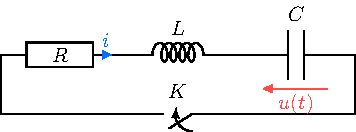
\includegraphics[width=.5\linewidth]{rlc_descendant}
% 	  \caption{Circuit.}
% 	  \label{fig:P1base}
% 	\end{figure}
% }
\enonce{%
	\noindent
	\begin{minipage}[c]{.45\linewidth}
		On considère le circuit RLC série représenté ci-contre.
		L'interrupteur $K$ est fermé à un instant $t=0$ choisi comme origine des
		temps. Le condensateur est initialement chargé~: $u(t=0)=u_0$.
	\end{minipage}
	\hfill
	\begin{minipage}[c]{.45\linewidth}
		~
		% \vspace{-15pt}
		\begin{center}
			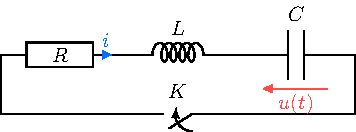
\includegraphics[width=\linewidth]{rlc_descendant}
			\captionof{figure}{Circuit.}
			\label{fig:P1base}
		\end{center}
	\end{minipage}
}

\QR[8]{%
	Établir l'équation différentielle vérifiée par $u(t)$ pour $t\geq 0$. La
	mettre sous la forme
	\[
		\dv[2]{u}{t} + \frac{\w_0}{Q}\dv{u}{t} + \w_0{}^{2}u = 0
	\]
	et donner les expressions de $\w_0$ et $Q$ en fonction de $R$, $L$ et $C$.
}{%
	~\\
	\vspace{-15pt}
	\begin{isd}
		Avec la loi des mailles,\\
		\begin{DispWithArrows}[fleqn, mathindent=2pt]
			u_L + u_R + u_C &= 0
			\notag
			\Arrow{$u_L = L \dv{i}{t}$\\et $u_R = Ri$}
			\\\Lra
			L \dv{i}{t} + Ri + u_C &= 0
			\notag
			\Arrow{$i = C \dv{u_C}{t}$}
			\\\Lra
			LC \dv[2]{u_C}{t} + RC \dv{u_C}{t} + u_C                   &= 0
			\notag
			\Arrow{forme\\canonique}
			\\
			\Lra \dv[2]{u_C}{t} + \frac{R}{L} \dv{u_C}{t} + \frac{1}{LC}u_C &= 0
			\label{eq:rlsimple}
		\end{DispWithArrows}
		\tcblower
		On détermine l'expression de $Q$ par identification~:
		\begin{DispWithArrows*}[fleqn, mathindent=20pt]
			\frac{\w_0}{Q} &= \frac{R}{L}
			\Arrow{$\DS\w_0 = \frac{1}{\sqrt{LC}}$}
			\\\Lra
			\frac{1}{Q \sqrt{LC}} &= \frac{R}{L}
			\Arrow{On isole $Q$}
			\\\Lra
			Q &= \frac{L}{R \sqrt{LC}}
			\Arrow{$L = \sqrt{L}^{2}$}
			\\\Lra
			\Aboxed{Q &= \frac{1}{R}\sqrt{\frac{L}{C}}}
		\end{DispWithArrows*}
	\end{isd}
}

%%%%%%%%%%%%%%%%%%%%%%%%%%%%%%%%%%%%

\QR[5]{%
	Montrer que le système répond différemment selon la valeur de $Q$. Nommer
	chaque régime possible, sans chercher à donner les formes de solutions
	correspondantes.
}{%
	% \ifstudent{
	% 	\vspace*{-\dimexpr\baselineskip+\abovedisplayskip\relax}
	% }
	~\\
	\vspace{-15pt}
	\begin{isd}
		Avec l'équation caractéristique~:
		\begin{gather*}
			r^2 + \frac{\w_0}{Q}r + \w_0{}^2 = 0
			\\\Ra
			\Delta =
			\left( \frac{\w_0}{Q} \right)^2 - 4\w_0{}^2 =
			\frac{\w_0{}^{2}}{Q^{2}}\left( 1-4Q^{2} \right)
		\end{gather*}
		Selon la valeur du discriminant, on aura différentes valeurs de $r$,
		doubles réelles, simple réelle ou doubles complexes. On a en effet, avec $Q >
			0$,
		\tcblower
		\begin{gather*}
			\Delta > 0
			\Lra
			\cancel{\frac{w_0{}^{2}}{Q^{2}}}\left( 1-4Q^{2} \right) >0
			\Lra
			4Q^2 < 1
			\Lra
			Q < \frac{1}{2}
		\end{gather*}
		\begin{description}
			\item[$\mathbf{Q > 1/2}$]~: régime \textbf{pseudo-périodique},
			racines complexes et oscillations décroissantes~;
			\item[$\mathbf{Q = 1/2}$]~: régime \textbf{critique}, racine double
			réelle~;
			\item[$\mathbf{Q < 1/2}$]~: régime \textbf{apériodique}, racines
			réelles et décroissance exponentielle sans oscillation.
		\end{description}
	\end{isd}
}

\enonce{
	On suppose $Q >1/2$ dans la suite.
}
\QR[4]{%
	Définir la pseudo-pulsation $\W$ des oscillations libres en fonction de
	$\w_0$ et $Q$. Définir aussi le temps caractéristique $\tau$ d'amortissement
	exponentiel des oscillations libres en fonction de $\w_0$ et $Q$.
}{%
	~\\
	\vspace{-15pt}
	\begin{isd}
		\begin{DispWithArrows*}[fleqn, mathindent=10pt]
			r_\pm & = \frac{-\frac{\w_0}{Q} \pm \jj\sqrt{-\D}}{2}
			\Arrow{On injecte $\Delta$}
			\\\Lra
			r_\pm &= -\frac{\w_0}{2Q} \pm
			\frac{\jj}{2} \sqrt{\frac{\w_0{}^{2}}{Q^{2}}\left( 4Q^{2}-1 \right)}
			\Arrow{On extrait $\frac{\w_0}{Q}$}
			\\\Lra
			r_\pm &= - \frac{\w_0}{2Q} \pm \jj \frac{\w_0}{2Q} \sqrt{4Q^{2}-1}
			\Arrow{On définit $\W$}
			\\\Lra
			r_\pm &= - \frac{\w_0}{2Q} \pm \jj\W
		\end{DispWithArrows*}
		\tcblower
		d'où la définition de $\W$~:
		\[
			\boxed{\W = \frac{\w_0}{2Q}\sqrt{4Q^{2}-1}}
		\]
		Ensuite, avec la forme générale de la solution on a
		\begin{equation*}
			u(t) = \exp \left(-\frac{\w_0}{2Q}t\right)
			\left[ A\cos(\Wt) + B\sin(\Wt) \right]
		\end{equation*}
		On remarque donc qu'on peut assimiler le terme à l'intérieur de
		l'exponentielle comme l'inverse d'un temps, c'est-à-dire qu'on définit
		$\tau$ comme la partie réelle des racines~:
		\[
			\boxed{\tau = \frac{2Q}{\w_0}}
		\]
	\end{isd}
	% L'énoncé attend sans doute le temps de relaxation $\tau = \frac{Q}{\w_0}$
	% mais la forme canonique en $\dv[2]{u}{t} + \dfrac{1}{\tau} \dv{u}{t} +
	% \w_0^2 u = 0$ n'est pas à connaître. 
}
\QR[9]{%
	Établir l'expression de $u(t)$ pour $t\geq 0$ en fonction de $u_0$, $\w_0$,
	$Q$ et $\w$, compte tenu des conditions initiales que vous expliciterez
	et justifierez.
}{%
	On a donc
	\[
		u(t) = \exr^{-t/\tau} \left[ A\cos(\Wt) + B\sin(\Wt) \right]
	\]
	\begin{itemize}
		\item On trouve $A$ avec la première condition initiale (condensateur
		      initialement chargé et tension condensateur continue)~:
		      \begin{gather*}
			      u(0) = u_0 = 1 \left[ A \cdot 1 + B \cdot 0 \right] = A
			      \quad \Ra \quad \boxed{A=u_0}
		      \end{gather*}
		\item On trouve $B$ avec la seconde CI (il n'y a pas de courant avant la
		      fermeture de $K$ et courant continu dans la bobine)~:
		      \begin{gather*}
			      \dv{u}{t} =
			      -\frac{\w_0}{2Q}\exp \left( -\frac{\w_0}{2Q}t \right)\times
			      \left[ A\cos(\Wt) + B\sin(\Wt) \right] +
			      \exp \left( -\frac{\w_0}{2Q}t \right)
			      \left[ -A\W\sin(\Wt) + B\W\cos(\Wt) \right]
			      \\\Ra
			      \dv{u}{t}\/(0) = - \frac{\w_0}{2Q}A + \W B = 0
			      \\\Lra
			      \boxed{B = \frac{\w_0}{2Q\W}u_0}
			      \\
			      \beforetext{Ainsi,}
			      \boxed{
				      u(t) = u_0\exr^{-t/\tau}
				      \left[ \cos(\Wt) + \frac{\w_0}{2Q\W}\sin(\Wt) \right]
			      }
		      \end{gather*}
	\end{itemize}
}

\enonce{
	On souhaite visualiser la tension $u(t)$ sur l'écran d'un oscilloscope dont
	l'entrée est modélisée par l'association en parallèle d'une résistance
	$R_0=\SI{1,0}{M\ohm}$ et d'une capacité $C_0=\SI{11}{p\farad}$.
}
\QR[5]{%
	Montrer que si l'on tient compte de l'oscilloscope, l'équation
	différentielle vérifiée par $u(t)$ devient:
	\[
		L(C+C_0)\dv[2]{u}{t }+
		\left(\frac{L}{R_0}+RC+RC_0\right)\dv{u}{t}+
		\left(1+\frac{R}{R_0}\right)u=0
	\]
}{%
	\noindent
	\begin{minipage}[t]{.30\linewidth}
		On commence par représenter le circuit en ajoutant en parallèle de $C$ la
		résistance $R_0$ et la capacité $C_0$.
		\begin{center}
			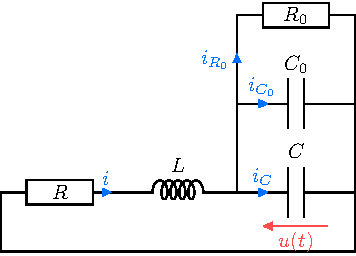
\includegraphics[width=\linewidth]{rlc_oscillo}
			\captionof{figure}{Circuit avec oscilloscope.}
			\label{fig:P1osci}
		\end{center}
	\end{minipage}
	\hfill
	\begin{minipage}[t]{.65\linewidth}
		Loi des nœuds~:
		\begin{DispWithArrows*}
			i &= i_{R_0} + i_{C_0} + i_C
			\Arrow{$i_C = C \dv{u}{t}$\\$i_{C_0} = C_0 \dv{u}{t}$\\$i_{R_0} =
					\frac{u}{R_0}$}
			\\\Lra
			i &= \frac{u}{R_0} + (C+C_0)\dv{u}{t}
		\end{DispWithArrows*}
		Dans la loi des mailles,
		\begin{DispWithArrows*}[fleqn, mathindent=-15pt]
			u_L + u_R + u &= 0
			\Arrow{$u_L = L \dv{i}{t}$\\$u_R = Ri$}
			\\\Lra
			L \dv{i}{t} + Ri + u &= 0
			\Arrow{$i = \frac{u}{R_0}$\\$ + (C+C_0)\dv{u}{t}$}
			\\\Lra
			\frac{L}{R_0} \dv{u}{t} + L(C+C_0) \dv[2]{u}{t} +
			\frac{R}{R_0}u + R(C+C_0) \dv{u}{t} + u &=0
			\Arrow{On factorise}
			\\\Lra
			\Aboxed{
				L(C+C_0)\dv[2]{u}{t} +
				\left(\frac{L}{R_0}+RC+RC_0\right)\dv{u}{t}+
				\left(1+\frac{R}{R_0}\right)u
				&= 0
			}
		\end{DispWithArrows*}
	\end{minipage}
}

\QR[7]{%
	Quelles relations qualitatives doivent vérifier $R$, $L$, $C$, $R_0$ et
	$C_0$ pour que la mise en place de l'oscilloscope ait une influence
	négligeable sur les oscillations étudiées~? Vérifier qu'avec les valeurs
	usuelles de $R$, $L$ et $C$ utilisées en travaux pratiques ces relations
	sont vérifiées.
}{%
	Pour que l'oscilloscope ait le moins d'influence possible sur les
	oscillations, il faut que les coefficients de l'équation différentielle
	précédente diffèrent le moins possible de ceux de l'équation
	différentielle~\eqref{eq:rlsimple}~:
	\begin{itemize}
		\item $C \gg C_0$; les capacités utilisées en T.P.\ sont de l'ordre du
		      $\si{nF}$ ou du $\si{\micro F}$. Comme $C_0=\SI{11}{pF}$, cette
		      condition est bien vérifiée~;
		\item $R \ll R_0$; les résistances utilisées en T.P.\ sont de l'ordre du
		      $\si{k\ohm}$. Comme  $R_0=\SI{1,0}{M\ohm}$ , cette condition
		      est bien vérifiée~;
		\item $\frac{L}{R_0} \ll RC$ soit $R_0 \gg \frac{L}{RC} \approx
			      \SI{e4}{\ohm}$~; cette condition est bien vérifiée.
	\end{itemize}
}

\QR[4]{%
	On définit le décrément logarithmique comme étant la quantité
	$d_m=\ln\dfrac{u(t)}{u(t+mT)}$ où $T=2\pi/\w$ et $m$ est un entier
	strictement positif. Exprimer $d_m$ en fonction de $m$ et de $Q$.
}{%
	En remarquant que $ \cos{(\W (t + T))} = \cos{(\W t + 2\pi)} = \cos{(\W
			t)}$, on montre facilement que $d_m =\ln { \left( \exp{\frac{\W_0 m T}{2Q}}
			\right) }$.
	On obtient donc~: $d_m = \dfrac{\w_0 m T}{2Q}$. En remplaçant $T$ par
	$\frac{2\pi}{\W}$ où $\W = \frac{\w_0}{Q} \sqrt{4Q^{2}-1}$, il vient~:
	\[
		\boxed{d_m = \frac{2 \pi m}{\sqrt{4Q^2-1}}}
	\]
}

\QR[2]{%
	On réalise un montage expérimental où le circuit RLC est excité par un
	générateur basses fréquences délivrant une tension créneau. Comment faut-il
	choisir le signal délivré par le générateur pour observer les oscillations
	libres du circuit~? Répondre en terme de la constante $\tau$ et à l'aide d'un
	schéma.
	\smallbreak
}{%
	\noindent
	\begin{minipage}[\sswitch{t}{c}]{.6\linewidth}
		Pour observer les oscillations il faut que la demi-période du signal délivré
		par le G.B.F.\ soit égale à quelques $\tau$. En effet, le régime permanent est
		atteint au bout d'approximativement $5\tau$. Une représentation avec le
		circuit RC est proposée ci-contre.
	\end{minipage}
	\hfill
	\begin{minipage}[\sswitch{t}{c}]{.38\linewidth}
		\ifstudent{
			\vspace{-40pt}
		}
		\begin{center}
			\includegraphics[width=\linewidth]{creneau_taugood}
			% \captionof{figure}{Accord entrée/sortie pour RC.}
			% \label{fig:taugoodRC}
		\end{center}
	\end{minipage}
}

\QR[3]{%
	La tension aux bornes du condensateur est enregistrée grâce à un logiciel
	d'acquisition. Le signal obtenu est représenté sur la
	figure~\ref{fig:P1graph}.
	\begin{figure}[htbp!]
		\centering
		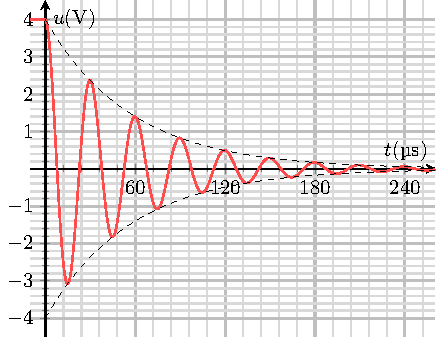
\includegraphics[width=.8\linewidth]{carac-rlc-15}
		\caption{Signal obtenu.}
		\label{fig:P1graph}
	\end{figure}
	Estimer le facteur de qualité $Q$ du circuit.
}{%
	On lit graphiquement $u(0)=4,0$V et $u(2T)=1,4$V. On peut alors calculer
	$d_2=\ln\dfrac{u(0)}{u(2T)}$.

	Comme $d_2= \frac{4 \pi }{\sqrt{4Q^2-1}}$, on en déduit~:
	$\boxed{ Q =
			\sqrt{ \frac{1}{4} + 4 \left( \frac{\pi}{d_2} \right) ^2}
		}
	$.
	Application numérique~: $\xul{Q = 6,0}$
}

\enonce{
	On suppose $Q\gg 1$: la dissipation d'énergie par effet Joule est traitée
	comme une perturbation par rapport au cas du circuit non dissipatif ($R=0$).
	On prendra alors $\w \approx \w_0$. On rappelle par ailleurs le
	développement limité de l'exponentielle en 0~:
	\[
		\exr^{x} \Sim_{x\to0} 1 + x
	\]
}
\QR[4]{%
Dans le cas où $R=0$, établir l'expression de la valeur moyenne temporelle
$\moy{\Ec}$ de l'énergie électromagnétique stockée dans le circuit.
}{%
Dans le cas où $R = 0$, le circuit est non dissipatif donc l'énergie
emmagasinée dans le condensateur et la bobine reste constante. On l'évalue
facilement en $t=0$~:
\[
	\Ec(t=0) = \frac{Cu_0^2}{2}
	\Ra
	\boxed{\moy{\Ec} = \frac{Cu_0^{2}}{2}}
\]
}

\QR[9]{%
	Dans le cas où $R\neq 0$, montrer qu'au premier ordre en $1/Q$, l'énergie
	$\Ec_J$ dissipée par effet \textsc{Joule} dans le circuit RLC, pendant une
	pseudo-période, vérifie la relation~:
	\[
		\Ec_J = \frac{2\pi}{Q}\moy{\Ec}
	\]
}{%
	Il faut évaluer l'énergie emmagasinée par le condensateur et la bobine à
	l'instant $t$~:
	\[
		\Ec(t) = \frac{Cu^2(t)}{2} + \frac{Li^2(t)}{2}
	\]
	Pour $Q \gg 1$, on a $\W \approx \w_0$ , l'expression de $u(t)$ devient~:
	\begin{DispWithArrows*}[groups]
		u(t) &= u_0 \exr^{-\frac{t}{\tau}}
		\left( \cos{(\w t)} + \frac{\w_0}{2Q\w} \sin{(\w t)} \right)
		\Arrow{$\W \approx \w_0$}
		\\\Lra
		u (t) &\approx u_0 \exr^{-\frac{t}{\tau}}
		\left( \cos{(\w_0 t)} + \frac{1}{2Q} \sin{(\w_0 t)} \right)
		\Arrow{$Q \gg 1 \Lra \frac{1}{Q} \approx 0$}
		\\\Lra
		\Aboxed{
			u(t) &\approx u_0 \exr^{-\frac{t}{\tau}} \cos{(\w_0 t)}
		}
		\Arrow{$i(t) = C \dv{u}{t}$}
		\\\Ra
		i(t) &= -Cu_0 \exr^{-\frac{t}{\tau}}
		\left( \w_0 \sin{(\w_0 t)} + \frac{1}{\tau} \cos{(\w_0 t)} \right)
		\Arrow{$\frac{1}{\tau} = \frac{\w_0}{2Q} \ll \w_0$}
		\\\Ra
		\Aboxed{i(t) &\approx -Cu_0 \w_0 \sin{(\w_0 t)} \exr^{-\frac{t}{\tau}}}
		\\\text{or}\qquad
		\Ec(t) &= \frac{Cu^2(t)}{2} + \frac{Li^2(t)}{2}
		\Arrow{On injecte}
		\\\Lra
		\Aboxed{\Ec(t) &= \frac{1}{2} C u_0^2 \exr^{ -\frac{2t}{\tau}}}
	\end{DispWithArrows*}
	En une pseudo-période $T$, l'énergie décroît de la quantité~:
	\begin{DispWithArrows*}
		\Delta_T{\Ec} &=
		\Ec(t) - \Ec(t+T)
		\\\Lra
		\Delta_T{\Ec} &=
		\frac{1}{2}Cu_0^2\exr^{-\frac{2t}{\tau}}
		\left( 1 - \exr^{ -\frac{2T}{\tau} } \right)
		\Arrow{$\tau = \frac{2Q}{\w_0}$}
		\\\Lra
		\Delta_T{\Ec} &=
		\frac{1}{2}Cu_0^2\exr^{-\frac{\w_0t}{Q}}
		\left( 1 - \exr^{ -\frac{\w_0T}{Q} } \right)
		\Arrow{$\W \approx \w_0$ et $\W T = 2\pi$}
		\\\Lra
		\Delta_T{\Ec} &=
		\frac{1}{2}Cu_0^2\exr^{-\frac{\w_0t}{Q}}
		\left( 1 - \exr^{ -\frac{2\pi}{Q} } \right)
		\Arrow{$\exr^{-\frac{2\pi}{Q}} \Sim_{Q\to\infty} 1 - \frac{2\pi}{Q}$}
		\\\Lra
		\Delta_T{\Ec} &\Sim_{Q\to\infty}
		\frac{1}{2}Cu_0^2 \underbracket[1pt]{\exr^{-\frac{\w_0t}{Q}}}_{\approx 1}
		\left( \cancel{1} - \left( \cancel{1} - \frac{2\pi}{Q} \right) \right)
		\Arrow{On simplifie}
		\\\Lra
		\Delta_T{\Ec} &\Sim_{Q\to\infty} \frac{2\pi}{Q} \moy{\Ec}
	\end{DispWithArrows*}
	Or, l'énergie dissipée par effet \textsc{Joule} en une pseudo-période
	correspond à l'énergie perdue par $L$ et $C$ pendant cette durée donc $\Ec_J =
		\Ec(t) - \Ec(t+T)$. Ainsi,
	\[
		\boxed{\Ec_J \approx \frac{2\pi}{Q}\moy{\Ec}}
	\]
}

% \resetQ
% \iftoggle{corrige}{}{%
%   \clearpage
% }
% \prblm[30]{Modélisation des mouvements d'une plateforme offshore}
% \enonce{
% On s’intéresse à la résolution d’une équation du mouvement dans une approche classique de la mécanique afin d’étudier le mouvement simplifié d’une plateforme en mer. Le modèle envisagé est un système à un degré de liberté considéré comme un oscillateur harmonique~: une masse est reliée à un ressort, avec amortissement.
%
% On considère le mouvement d’une plateforme en mer soumise à un courant marin. Sa partie supérieure de masse $m = \SI{110}{tonnes}$ est considérée comme rigide et le mouvement principal de la plateforme a lieu suivant $x$ (cf figure 1(a)). Afin d’étudier le mouvement de cette plateforme, on la représente par une masse $m$, liée à un ressort de 
% constante de raideur $k$ et à un amortisseur de constante d’amortissement $\gamma$ comme schématisé sur la figure 1(b). 
% La masse se déplace selon une seule direction, parallèle à l’axe $Ox$ en fonction du temps $t$. Ainsi, les projections sur l’axe $Ox$ de la position, de la vitesse et de l’accélération de la masse en fonction du temps sont notées respectivement $x(t)$, $\xp(t)$ et $\xpp(t)$. Le vecteur unitaire de l’axe $Ox$ est noté $\vv{i}$.
%
% \begin{figure}[htbp!]
%   \centering
%   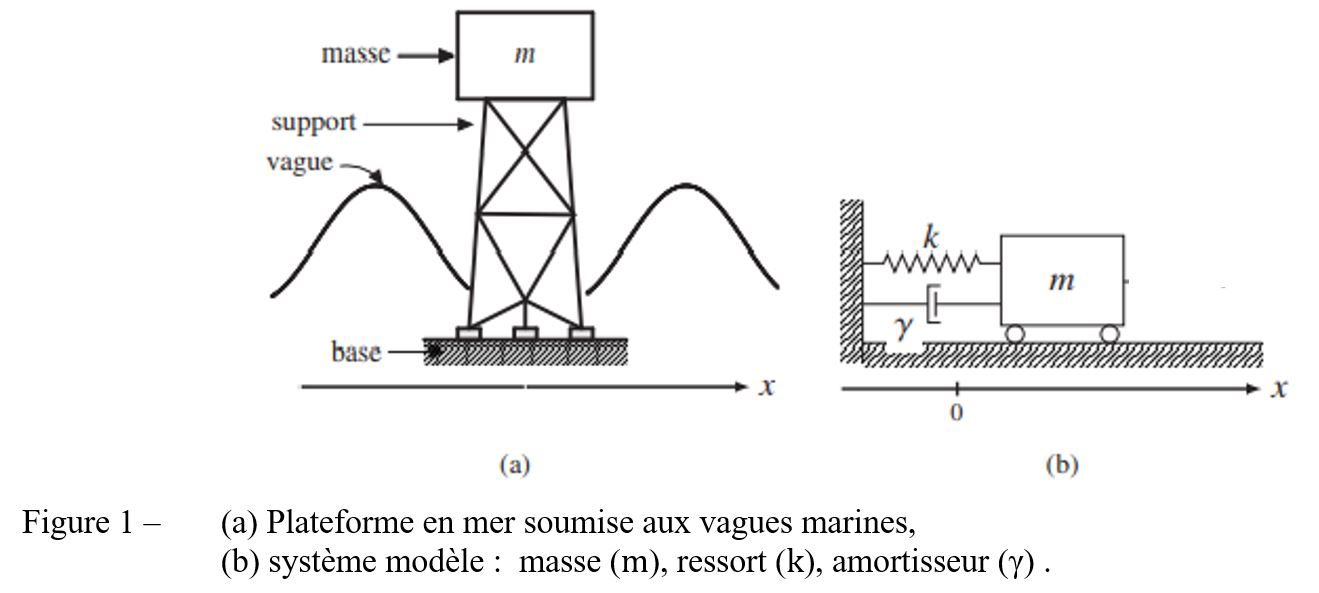
\includegraphics[width=.9\linewidth]{P2base}
% \end{figure}
%
% La masse se déplace sur la base horizontale sans frottements sur le support. La position d’équilibre de la masse sera choisie à $x = 0$.
%
% La force totale $\vv{F_{tot}}$ agissant sur la masse correspond à la réaction normale à la base horizontale $\vv{R_N}$, à la force de frottement $\vv{F_d}= - \gamma \vv{v}$  où $\gamma$ est la constante d’amortissement positive, permettant  de prendre en compte l’effet de l’eau environnante, à la force de rappel $\vv{F_k}$ du ressort et au poids $\vv{P}$ de la masse $m$.
% }
%
% \QR[0]
% {Etablir l’équation différentielle du mouvement de la masse $m$ et la mettre sous la forme~:
%
% \centersright{$\xpp+2\xi\w_0 \xp+{\w_0}^2 x=0$}{(équation 1)}
%
% \noindent
% On exprimera $\w_0$ et $\xi$ en fonction de $k$, $m$ et $\gamma$. On rappelle que $\xi =Q/2$.}
% {
% \begin{itemize}
% \item Référentiel d'étude: Référentiel terrestre $\mathcal{R}(O, x, y)$ supposé galiléen.
% \item Base de projection~: Base cartésienne $(O, x, y)$ de vecteurs unitaires $\vv{i}$ et $\vv{j}$. L'origine est prise à la position d'équilibre comme indiqué dans l’énoncé. $\vv{j}$ est orienté vers le haut.
% \item Système: la plateforme $M$ de masse $m$. 
% \item Bilan des forces: 
% \begin{enumerate}
% \item Poids~: $\vv{P}=m\vv{g} = - mg\vv{j}$ .
% \item Réaction du support: $\vv{R_N}=R_N\vv{j}$~; $R$ est orthogonale au déplacement car mouvement sans frottements.
% \item Force de rappel du ressort~: $\vv{F}= - k \left(l-l_o\right)\vv{i} = - k x \vv{i}$ , car $\ell = \ell_0 + x$.
% \item Force de frottement $\vv{F_d}=-\gamma\vv{v}=-\gamma\xp\vv{i}$ .
% \end{enumerate}	
% \end{itemize}
%
% 2ème loi de Newton (principe fondamental de la dynamique):
%
% \centers{	$\sum{\vv{F}=m\vv{a}=m\dv{\vv{v}}{t}}$}
%
% \leftcenters{	d’où}{ $\vv{P}+\vv{R_N}+\vv{F}+\vv{F_d}=m\vv{a}$} 
%
% 	\noindent
% 	avec $\vv{a}=\xpp\vv{i}$ car le mouvement se fait sur $Ox$.
% 	Projetons sur les 2 axes.
%
% 	 \leftcentersright{Sur $\vv{i}$}{$m\xpp+kx+\gamma\xp=0$}	{(équation du mouvement)}
%
%       \leftcentersright{Sur $\vv{j}$~:} {$R_N- mg = 0$} {(pas de mouvement sur $Oy$)}
%
%       \noindent
% Reprenons la première équation en la mettant sous forme canonique, il vient~: 
%
% \centers{$\xpp+\frac{\gamma}{m}\xp+\frac{k}{m}x=0$}
%
% \leftcenters{De la forme}{  $\xpp+2\xi\w_0\xp+\w_0^2x=0$}
%
%
% \leftcenters{avec} {$\w_0=\sqrt{\frac{k}{m}} \quad \text{et} \quad 2\xi\w_0=\frac{\gamma}{m}$}
%
% \leftcenters{Soit} {$\xi=\frac{\gamma}{2m\w_0}=\frac{\gamma}{2m}\sqrt{\frac{m}{k}} = \frac{\gamma}{2}\sqrt{\frac{1}{mk}}$}
% }
%
% \QR[0]
% {Dans le cas où  $\xi < 1$, justifier que $x\left(t\right)$ peut prendre la forme suivante~:
%
% \centersright{$x\left(t\right)=\exr^{-\xi\w_0 t}[A \cos(\W t)+B \sin(\W t)]$}{(équation 2)}
%
% où $\W$ est la pseudo-pulsation que l’on exprimera en fonction de $\w_0$ et $\xi$.
% De plus, en remarquant qu’à $t=0$, $x\left(0\right)=x_0$ et $\xp\left(0\right)=v_0$, déterminer les expressions des deux coefficients réels $A$ et $B$ en fonction de $x_0$, $v_0$ , $\xi$ , $\w_0$ et $\W$}
% {
% Solution de cette équation différentielle d’ordre 2~:
%
%  \centers{$\xpp+2\xi\w_0\xp+\w_0^2x=0$}
%
% \leftcenters{Equation caractéristique associée~:} {$r^2+2\xi\w_0 \, r+{\w_0}^2=0$}
%
%
% \leftcenters{Discriminant~: }{$\Delta=4\xi^2\, {\w_0}^2-4{\w_0}^2=4 {\w_0}^2(\xi^2-1)$}
%
% \noindent
% Ici, $\xi<1$, donc $\Delta <0$~; C’est un régime pseudo-périodique.	Les solutions de l’équation caractéristique sont alors~: 
%
% \centers{$r_{1,2}=\frac{-2\xi\w_0 \pm i\sqrt{-\Delta}}{2}= - \w_0\pa{\xi \pm i \sqrt{1-\xiç 2}}$}
%
% \noindent
% On pose   $\alpha=\frac{-b}{2a}  = -\xi\w_0$	et $\W=\frac{\sqrt{-\Delta}}{2a}= \w_0 \, \sqrt{1-\xi^2}$ la pseudo–pulsation. Alors
%
% \centers{ $x\left(t\right)=\exp{\left(\alpha t\right)}\left[A \cos\left(\W t\right)+B \sin\left(\W t\right)\right]$}
%
% \leftcenters{Soit }{$x\left(t\right)=e^{-\xi\w_0t}[A \cos\W t+B \sin(\W t)]$}
%
% De plus, les conditions initiales sont, à $t=0$, $x\left(0\right)=x_0$ , donc $A=x_0$. 
% Calculons de plus la dérivée 
%
% \centers{$\xp\left(t\right)=\left[-A\W\sin{\left(\W t\right)+}B\W \cos\left(\W t\right)\right] \exp{\left(\alpha t\right)}+\alpha\left[A\cos{\left(\W t\right)+}B \sin\left(\W t\right)\right]\exp(\alpha t)$}
%
%
% \leftcenters{Nouvelle condition initiale~:} {$\xp\left(0\right)=v_0$} 
%
% \leftcenters{Donc}{ $B\W+\alpha A=v_0$}
%
% \leftcenters{ Soit }{$B=\frac{v_0-\alpha A}{\W}=\frac{v_0+\xi\w_0x_0}{\W}=\frac{v_0+\xi\w_0x_0}{\w_0\sqrt{1-\xi^2}}$}
% }
%
% \QR[0]
% {Montrer que l’on peut aussi obtenir une forme de la solution du type~:
%
% \centersright{$x\left(t\right)=X_m \exr^{-\xi\w_0t}\cos{(} \mathrm{\W t}+\varphi)$}{(équation 3)} 
%
% \noindent                                                                  
% On exprimera $X_m$ et $\varphi$ en fonction de $A$ et $B$. Quelques outils mathématiques sont donnés en fin de cet exercice. }
% {
% \leftcenters{On nous donne} {$x\left(t\right)=X_me^{-\xi\w_0t}\cos{(}\W t+\varphi)$}
%
% \leftcenters{Et} {$cos\left(a+b\right)=\cos{\left(a\right)}\cos{\left(b\right)}-\sin{\left(a\right)}\sin(b)$}
%
% \leftcenters{Soit}{ $x\left(t\right)=X_me^{-\xi\w_0t}\left[\cos{(\W t)}\cos{(\varphi)}-\sin{\left(\W t\right)\sin{(\varphi)}}\right]$}
%
%
% Par identification avec $x\left(t\right)=e^{-\xi\w_0t}[Acos\W t+Bsin(\W t)]$, il vient		 
%
% \centers{$X_m\cos{(\varphi)}=A \quad \text{et} \quad -X_m\sin\left(\varphi\right)=B$}
%
%
%
% \leftcenters{Ainsi }{$\tan{\left(\varphi\right)=-\frac{B}{A}} \quad \text{et} \quad A^2+B^2=X_{m}^2(\cos^2\left(\varphi\right)+\sin^2\left(\varphi\right))=X_{m}^2$}
%
% \leftcenters{D’où}{ $\varphi=-\arctan\left(\frac{B}{A}\right) \quad \text{et} \quad X_m=\sqrt{A^2+B^2}$}
% }
%
% \QR[0]
% {Représenter qualitativement $x\left(t\right)$ en fonction de $t$ et indiquer sur le tracé $X_m e^{-\xi\w_0t}$ , $x_0$ et $T={2\pi}/{\W}$ la pseudo-période.}
% {
% Allure du graphe ci-contre~: 
%
% \begin{figure}[htbp!]
%   \centering
%   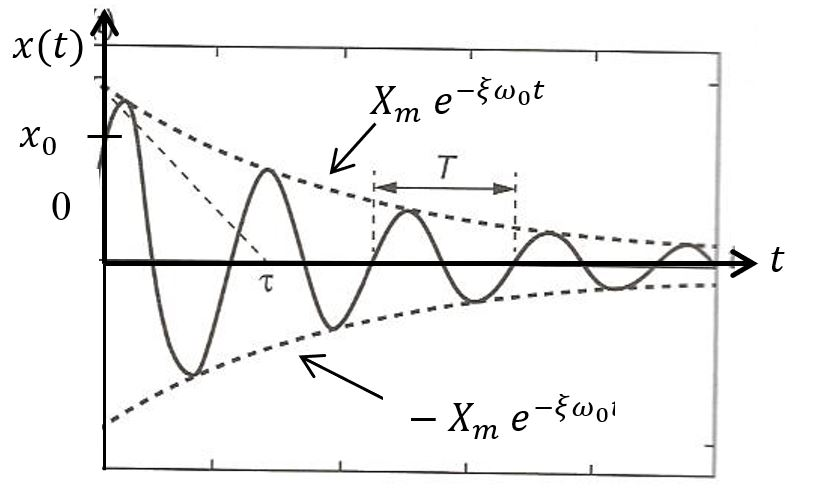
\includegraphics[width=.6\linewidth]{P1corr.jpg}
%   \caption{Allure du graphe. On note la dérivée non nulle en 0.}
%   \label{fig:P1corr}
% \end{figure}
%
% }
%
% \QR[0]
% {Justifier qualitativement que l’énergie mécanique $E(t)$ est une fonction décroissante de $t$. À quoi cela est-il dû~?}
% {
% A cause des frottements, l’énergie mécanique $E(t)$ est une fonction décroissante de $t$.
% }
%
% \QR[0]
% {On envisage deux temps successifs $t_1$ et $t_2$ pour lesquels les déplacements sont $x_1$ et $x_2$, tels que $t_2 > t_1$ 
% et $t_2-t_1=T$ , où $T$ est la période des oscillations amorties. 
% En utilisant l’équation (3) et en considérant que $\xi \ll 1$, montrer que~:            
%
% \centers{$\ln{\left(\frac{x_1}{x_2}\right)} \approx 2\pi\xi$}
% }
% {
% Cela fait penser au décrément logarithmique~:
%
% \centers{
%  $\delta=\ln{\frac{x\left(t\right)}{x\left(t+T\right)}=\ln{\left(\frac{x_1}{x_2}\right)}=\ln{\frac{{X_me}^{\alpha t}\cos{\left(\W t+\varphi\right)}}{{X_me}^{\alpha(t+T)}\cos{\left(\W(T+t)+\varphi\right)}}=\ln{\left(e^{-\alpha T}\right)}}}$}
%
%  \noindent
%   car cosinus est une fonction périodique de période $T$.
% Soit~: 
%
% \centers{$\delta=\ln{\left(\frac{x_1}{x_2}\right)}=-\alpha T=\xi\w_0 T=\xi\w_0\frac{2\pi}{\W}=\xi\w_0\frac{2\pi}{\w_0\sqrt{1-\xi^2}}= \xi\frac{2\pi}{\sqrt{1-\xi^2}}$}
%
%
% Or par hypothèse,  $\xi \ll 1$ , donc $1-\xi^2\approx 1$~; Alors
%
% \centers{ $\ln{\left(\frac{x_1}{x_2}\right)}\approx2\pi\xi$}
% }
%
% \QR[0]
% {Toujours dans le cas où $\xi\ll 1$, le relevé du déplacement horizontal de la plateforme en fonction du temps 
% est représenté en figure 2 ci-dessous. En utilisant les deux points qui sont indiqués sur la figure 2, déterminer les valeurs numériques de $k$, $\xi$ et $\gamma$ (avec leurs unités). Comment ce tracé serait-il modifié si $\xi$ augmentait (un rapide graphique peut permettre d’être plus explicite)~? 
%
% \begin{figure}[htbp!]
%   \centering
%   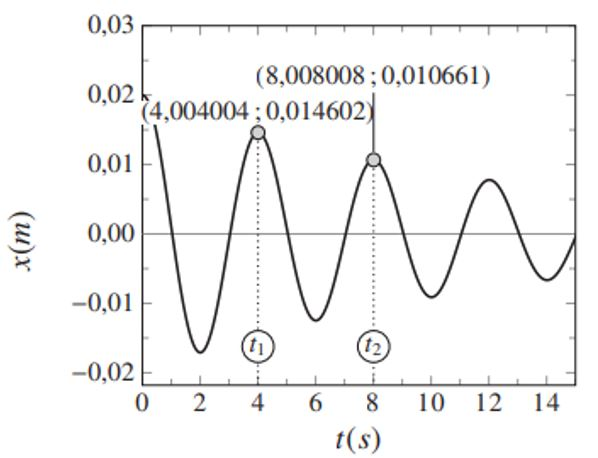
\includegraphics[width=.6\linewidth]{P2graph}
%   \caption{ Relevé du déplacement horizontal $x$ (en m) de la plateforme de
%   masse $m = \SI{110}{tonnes}$ en fonction du temps $t$ (en s). Les deux temps
% $t_1$ et $t_2$ mentionnés en question Q6 sont indiqués.}
%   \label{fig:P2graph}
% \end{figure}
%
% }
% {
% On lit $x_1=\SI{0,014602}{m}$ et $t_1=\SI{4,004004}{s}$, puis $x_2=\SI{0,010661}{m}$ et $t_2=\SI{8,008008}{s}$.
% 	D’après l’énoncé, on a  $T=t_2-t_1$ et comme $\xi \ll 1$ alors
%
%  \centers{$\w_0\approx\W=\frac{2\pi}{T}=\frac{2\pi}{t_2-t_1}$}
%
%
%  \leftcenters{ car $\W  =\w_0\sqrt{1-\xi^2}$. De plus,}{ $\w_0=\sqrt{\frac{k}{m}}$}
%
% \leftcenters{ Donc}{ $k=m\w_0^2=m\frac{4\pi^2}{\left(t_2-t_1\right)^2} = 110.{10}^3\frac{4\pi^2}{\left(8,008008-4,00400\right)^2} = \SI{2,71e5} {N.m^{-1}}$}
%
%  \noindent
% 	D’autre part d’après Q6, 
%
% \centers{$\ln{\left(\frac{x_1}{x_2}\right)}=2\pi\xi$}
% \leftcenters{Soit }{$\xi=\frac{\ln{\left(\frac{x_1}{x_2}\right)}}{2\pi} = \frac{\ln{\left(\frac{0,014602}{0,010661}\right)}}{2\pi} = \num{5,01e-2}$}
%
% \noindent
% Remarque~: on trouve en effet comme attendu $\xi\ll1$. C'est cohérent. 
%
% \medskip
%
% \leftcenters{Enfin, d’après Q1,} {$\xi=\frac{\gamma}{2}\sqrt{\frac{1}{mk}}$}
%
% \leftcenters{Soit}{ $\gamma=2\xi\sqrt{mk} = 2\times5.01.{10}^{-2}\sqrt{110.{10}^3\times2,71.{10}^5} = \SI{1,73e4} {N.s.m^{-1}}$} .
%
% \noindent
% 	Si $\xi$ augmentait, l’amortissement augmenterait, la décroissance exponentielle serait plus rapide, on 
% verrait moins d’oscillations et la pseudo-pulsation $\W$  diminuerait et la pseudo-période $T={2\pi}/{\W}$ augmenterait.
% }
%
% \enonce
% {
% \medskip
%
% \noindent
% \underline{Outils mathématiques}~: 		
%
% \centers{$cos\left(a+b\right)=\cos{\left(a\right)}\cos{\left(b\right)}-\sin{\left(a\right)}\sin(b) \quad \text{et} \quad
% 					{cos}^2\left(\alpha\right)+{sin}^2\left(\alpha\right)=1$} 
% }

\iftoggle{corrige}{}{%
	\clearpage
}
\resetQ
\prblm[58]{Assemblages de ressorts}
\enonce{
	\noindent
	\begin{minipage}[t]{.48\linewidth}
		Pour un TIPE, un-e étudiant-e a besoin d'un ressort de raideur
		$\SI{15}{\N\per\m}$. Malheureusement, le laboratoire du lycée ne possède que
		des ressorts de raideur $k_1=\SI{10}{\N\per\m}$ et $k_2=\SI{20}{\N\per\m}$.
		En revanche, tous les ressorts ont la même longueur à vide
		$\ell_0=\SI{10}{\cm}$.
		\bigbreak
		L'étudiant-e décide alors d'assembler les ressorts pour obtenir la raideur
		qu'iel souhaite. Iel hésite cependant entre un assemblage en série ou en
		parallèle, voir Figures~\ref{fig:assem_serie} et~\ref{fig:assem_para}
		ci-contre.
		\bigbreak
		Iel mène donc une étude des deux assemblages pour voir
		comment ils se comportent. Iel dispose d'une masse $m=\SI{100}{g}$ repérée par
		le point $M$, considéré comme un point matériel. On négle les masses des
		ressorts.
	\end{minipage}
	\begin{minipage}[t]{.24\linewidth}
		\vspace{-5pt}
		\begin{center}
			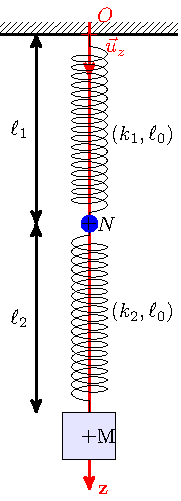
\includegraphics[height=5cm]{ressorts_verticaux_serie.pdf}
			\captionof{figure}{Assemblages en série}
			\label{fig:assem_serie}
		\end{center}
	\end{minipage}
	\begin{minipage}[t]{.24\linewidth}
		\vspace{-5pt}
		\begin{center}
			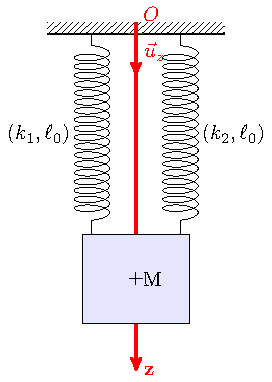
\includegraphics[height=5cm]{ressorts_verticaux_parallele.pdf}
			\captionof{figure}{Assemblages en parallèle}
			\label{fig:assem_para}
		\end{center}
	\end{minipage}
}

\partie{Assemblage en série}

\enonce{%
	Dans ce montage, le premier ressort est accroché au niveau du support fixe en un
	point noté O. Le second ressort est accroché au premier en un point N. Pour
	mener l'étude, on considèrera que le point N possède une masse $m'$. On note
	O$z$ la verticale descendante, dirigée par le vecteur unitaire $\uz$,
	orienté vers le bas (cf.\ Figure~\ref{fig:assem_serie}).
}

\ifcorrige{
	\begin{center}
		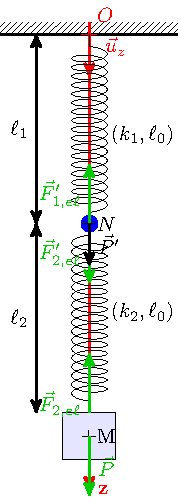
\includegraphics[height=7cm]{ressorts_verticaux_serie_corrige.pdf}
		\captionof{figure}{Assemblages en série}
		\label{fig:assem_serie-corr}
	\end{center}
}
\QR[4]{%
	Faire le bilan des forces s'exerçant sur le point M, les représenter sur un
	schéma et les exprimer en fonction des paramètres du problème.
}{%
	\label{q:bdf_serie}
	\begin{itemize}
		\bitem{BDF~:}
		\[
			\begin{array}{ll}
				\textbf{Poids}     & \Pf = mg\uz
				\\
				\textbf{Ressort 2} & \vv{F}\ind{2, el} = -k_2(\ell_2-\ell_0)\uz
			\end{array}
		\]
	\end{itemize}
	En effet, si on suppose que le ressort est étiré, il exerce sur la masse une
	force vers le haut, donc selon $-\uz$. Or dans ce cas, $\Delta \ell_2 =
		\ell_2-\ell_0>0$ et l'expression précédente avec le signe moins fournit bien
	une force orientée selon $-\uz$. Voir Figure~\ref{fig:assem_serie-corr}
}

%%%%%%%%%%%%%%%%%%%%%%%%%%%%%%%%%%%%

\QR[3]{%
	\label{q:leq_serie}
	En déduire l'expression de la longueur à l'équilibre $\ell\ind{2,eq}$ du ressort
	$2$ (celui placé en bas) en fonction des paramètres du problème. Faire
	l'application numérique.
}{%
	À l'équilibre, la somme des forces extérieures appliquées à la masse est nulle~:
	\begin{DispWithArrows*}[]
		\vv{F}\ind{2,el} + \vv{P} &= \vv{0}
		\Arrow{On remplace}
		\\\Lra
		-k_2(\ell_{2,eq}-\ell_0)\uz + mg\uz &= \vv{0}
		\Arrow{On multiple par $\cdot \uz$}
		\\\Lra
		-k_2(\ell_{2,eq}-\ell_0) + mg &= 0
		\Arrow{On isole}
		\\\Lra
		\Aboxed{\ell_{2,eq} &= \ell_0 + \dfrac{mg}{k_2}}
		\Arrow{Calcul}
		\\
		\makebox[0pt][l]{$\phantom{\AN}\xul{\phantom{\ell\ind{2,eq} = \SI{15}{cm}}}$}
		\AN
		\ell\ind{2,eq} &= \SI{15}{cm}
	\end{DispWithArrows*}
}

%%%%%%%%%%%%%%%%%%%%%%%%%%%%%%%%%%%%

\QR[6]{%
	Faire le bilan des forces s'exerçant sur le point $N$, les représenter sur le
	même schéma et les exprimer en fonction des paramètres du problème.
}{ %%%%%%%%%%%%%
	\begin{itemize}
		\bitem{BDF~:}
		\[
			\begin{array}{ll}
				\textbf{Poids}     & \Pf = m'g\uz
				\\
				\textbf{Ressort 2} & \vv{F'}\ind{2, el} = k_2(\ell_2-\ell_0)\uz
				\\
				\textbf{Ressort 1} & \vv{F'}\ind{1, el} = -k_1(\ell_1-\ell_0)\uz
			\end{array}
		\]
	\end{itemize}
	En effet, si on suppose que le ressort $2$ est étiré, il exerce sur la masse
	une force vers le bas, donc selon $+\uz$. Or dans ce cas, $\Delta \ell_2
		= \ell_2-\ell_0>0$ et l'expression précédente avec le signe plus fournit bien
	une force orientée selon $+\uz$. La justification du signe de la force
	$\vv{F}'\ind{1,el}$ est identique à celle de la question
	\ref{q:bdf_serie}.
}

%%%%%%%%%%%%%%%%%%%%%%%%%%%%%%%%%%%%

\QR[4]{%
	En déduire que la longueur à l'équilibre $\ell\ind{1,eq}$ du ressort $1$
	(celui placé en haut) est donnée par~:
	\[
		\ell\ind{1,eq} = \ell_0 + \dfrac{(m+m')g}{k_1}
	\]
}{
	%%%%%%%%%%%%%
	À l'équilibre, la somme des forces extérieures appliquées à la masse est nulle~:
	\begin{DispWithArrows*}[groups]
		\vv{F}'\ind{1,el} + \vv{F}'\ind{2,el} + \vv{P}' = \vv{0} & \Lra -k_1(\ell_{1,eq}-\ell_0)\uz  + k_2(\ell_{2,eq}-\ell_0)\uz + m'g\uz = \vv{0} \\
		& \Lra -k_1(\ell_{1,eq}-\ell_0)+k_2(\ell_{2,eq}-\ell_0) + m'g = 0                                 \\
		& \Lra k_1(\ell_{1,eq}-\ell_0) =  k_2(\ell_{2,eq}-\ell_0) + m'g                                   \\
		& \Lra \ell_{1,eq} = \ell_0 + \dfrac{k_2(\ell_{2,eq}-\ell_0) + m'g}{k_1}
		\Arrow{\ref{q:leq_serie} $\Ra k_2(\ell_{2,eq}-\ell_0) = mg$} \\
		& \Lra \boxed{\ell_{1,eq} = \ell_0 + \dfrac{(m+m')g}{k_1}}
	\end{DispWithArrows*}
}

\QR[2]{%
	Commenter la formule précédente.
}{%
	Du point de vue du ressort $1$, tout se passe comme si on avait accroché une
	masse de valeur $m+m'$. En effet, pour le ressort, que cette masse soit d'un
	seul tenant ou constituée de deux masses (et un ressort de masse nulle) ne
	change rien.
}

%%%%%%%%%%%%%%%%%%%%%%%%%%%%%%%%%%%%%
%\QR[0]{%
%En utilisant le principe fondamental de la dynamique appliqué au ressort 2 supposé de masse nulle, trouver une relation entre la force appliquée par le ressort 2 sur le point N et la force appliquée par le ressort 2 sur le point M. Commenter.
%}{%%%%%%%%%%%%%
%Pas de corrigé.
%}
%%%%%%%%%%%%%%%%%%%%%%%%%%%%%%%%%%%%

\QR[4]{%
	Déterminer l'expression de l'altitude $z\ind{eq}$ du point $M$. Simplifier la
	formule dans le cas où le point $N$ possède une masse nulle ($m'=0$).
}{%
	Dans la configuration établie par l'énoncé, on a $z=\ell_1+\ell_2$. À
	l'équilibre, on a alors~:
	\[
		z\ind{eq}=\ell_{1,eq}+\ell_{2,eq} =
		\ell_0 + \dfrac{(m+m')g}{k_1} + \ell_0 + \dfrac{mg}{k_2}
		\qso
		\boxed{z\ind{eq} = 2\ell_0  + \dfrac{(m+m')g}{k_1} + \dfrac{mg}{k_2}}
	\]
	En tenant compte d'une masse nulle pour le point $N$, on obtient~:
	\[
		\boxed{z\ind{eq} = 2\ell_0  + \pa{\dfrac{1}{k_1} + \dfrac{1}{k_2}}mg}
	\]
}

\QR[3]{%
	Par analogie avec le résultat que vous obtiendriez si la masse $m$ n'était
	accrochée qu'à un seul ressort de raideur $K$ et de longueur à vide $\ell_0$,
	déterminer les caractéristiques ($K$ et $\ell_0$) de ce ressort équivalent aux
	deux ressorts accrochés en série.
}{%%%%%%%%%%%%%
	Le cas d'un seul ressort vertical donne~:
	\[
		z\ind{eq} = \ell_0 + \dfrac{1}{K}mg
	\]
	En identifiant les deux formules terme à terme, on a~:
	\[
		\boxed{\ell_0 = 2\ell_0}
		\qet
		\dfrac{1}{K} = \dfrac{1}{k_1} + \dfrac{1}{k_2}
		\qso
		\boxed{K = \dfrac{k_1k_2}{k_1+k_2}}
	\]
}

\QR[2]{%
	Montrer que cet assemblage ne peut pas satisfaire l'étudiant-e pour son TIPE.
}{%
	On calcule $K$ avec les valeurs fournies~: $\xul{K = \SI{6,7}{\N\per\m}}$.
	C'est trop faible.
}

\partie{Assemblage en parallèle}

\enonce{%
	Dans ce montage, les deux ressorts sont accrochés au même support fixe et à la
	masse $m$. On note toujours O$z$ la verticale descendante, dirigée par le
	vecteur unitaire $\uz$, orienté vers le bas (cf.\
	Figure~\ref{fig:assem_para}).
}

\ifcorrige{
	\begin{center}
		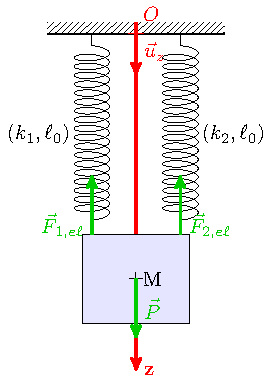
\includegraphics[height=7cm]{ressorts_verticaux_parallele_corrige.pdf}
		\captionof{figure}{Assemblages en parallèle}
		\label{fig:assem_para-corr}
	\end{center}
}

\QR[7]{%
	Expliciter le lien entre $\ell_1$, $\ell_2$ et $z$, puis faire le bilan des
	forces qui s'exercent sur le point $M$ et les représenter sur un schéma.
}{%
	\begin{itemize}
		\bitem{BDF~:}
		\[
			\begin{array}{ll}
				\textbf{Poids}     & \Pf = mg\uz
				\\
				\textbf{Ressort 1} & \vv{F}\ind{1, el} = -k_1(\ell-\ell_0)\uz
				\\
				\textbf{Ressort 2} & \vv{F}\ind{2, el} = -k_2(\ell-\ell_0)\uz
			\end{array}
		\]
	\end{itemize}
	On a tenu compte du fait qu'ici $\ell_2=\ell_1 = \ell$ et on a mis le signe
	des forces en accord avec ce qui a déjà été établi précédemment.
}

\QR[10]{%
	Établir l'équation du mouvement du point $M$ et la mettre sous forme
	canonique. Vous prendrez soin de détailler extensivement le cadre mécanique
	nécessaire à cette étude.
}{%
	\ifstudent{
		~\\
		\vspace{-15pt}
	}
	\begin{isd}[lefthand ratio=.35]
		\begin{itemize}
			\bitem{Système~:} \{point M\} de masse $m$
			\bitem{Référentiel~:} $\Rc\ind{lab}$ supposé galiléen
			\bitem{Repère~:} $(\Or,\uz)$ avec $\uz$ vers le bas
			\bitem{Repérage~:}
			\begin{align*}
				\OM(t) & = z\uz
				\\
				\vf(t) & = \zp\uz
				\\
				\af(t) & = \zpp\uz
			\end{align*}
		\end{itemize}
		\tcblower
		\begin{itemize}
			\bitem{PFD~:}
			\begin{DispWithArrows*}[fleqn, mathindent=0pt]
				m\af &= \Pf + \Ff\ind{1,el} + \Ff\ind{2,el}
				\Arrow{$\cdot \uz$ et $\ell = z$}
				\\\Lra
				m\zpp &= -k_1(z-\ell_0) -k_2(z-\ell_0) + mg
				\Arrow{On simplifie}
				\\\Lra
				m\zpp + (k_1+k_2)z &= (k_1+k_2)\ell_0 + mg
				\Arrow{Forme canonique}
				\\\Lra
				\Aboxed{
					\zpp + \dfrac{k_1+k_2}{m} z &=
					\dfrac{k_1+k_2}{m}\left(\ell_0 + \dfrac{mg}{k_1+k_2}\right)
				}
			\end{DispWithArrows*}
		\end{itemize}
	\end{isd}
	\bigbreak
	On pose $\boxed{\w_0 = \sqrt{\dfrac{k_1+k_2}{m}}}$ et $\boxed{z\ind{eq}=\ell_0
			+ \dfrac{mg}{k_1+k_2}}$~:
	\[
		\boxed{\zpp + \w_0^2 z = \w_0^2 z\ind{eq}}
		\label{eq:P2_harmo}
	\]
}

\QR[2]{%
	Déterminer les caractéristiques $K$ et $\ell_0$ du ressort équivalent aux
	deux ressorts accrochés en parallèle.
}{%
	On a déjà traité le cas d'un seul ressort dans la première partie du sujet. On
	constate qu'on a ici exactement la même équation que pour un seul ressort avec
	$\boxed{\ell_0 = \ell_0}$ et $\boxed{K = k_1+k_2}$.
}

%%%%%%%%%%%%%%%%%%%%%%%%%%%%%%%%%%%%

\QR[2]{%
	Montrer que cet assemblage ne peut pas satisfaire l'étudiant-e pour son TIPE.
}{%
	Avec cet assemblage, l'étudiant-e obtient un système équivalent à un ressort
	de raideur $\xul{K = \SI{30}{\N\per\m}}$, soit une raideur deux fois trop
	élevée.
}

\partie{Assemblage complexe}

%%%%%%%%%%%%%%%%%%%%%%%%%%%%%%%%%%%%

\QR[9]{%
	Déterminer un assemblage équivalent à un ressort ayant la raideur souhaité par
	l'étudiant-e. Faire un schéma de la situation proposée.
}{%
	\noindent
	\begin{minipage}[t]{.75\linewidth}
		\begin{itemize}
			\item l'assemblage en série donne ici une raideur deux fois trop élevée~;
			\item l'assemblage en parallèle peut permettre de diviser par deux la raideur.
		\end{itemize}
		En effet, dans la formule obtenue pour l'assemblage en série, on avait
		$K=\frac{k_1k_2}{k_1+k_2}$. Avec $k_1 = k_2$, cette formule devient $K =
			\frac{k_1^2}{2k_1} = \frac{k_1}{2}$. Un assemblage série de deux ressorts
		identiques permet bien de diviser par deux la raideur.
		\bigbreak
		On peut donc envisager le montage suivant~: on fabrique deux assemblages en
		parallèle identiques, chacun avec un ressort de raideur
		$k_1=\SI{10}{\N\per\m}$ et un ressort de raideur $k_2=\SI{20}{\N\per\m}$. Ces
		assemblages sont chacun équivalent à un ressort de raideur $k_3
			=\SI{30}{\N\per\m}$ d'après les résultats précédents.
		\bigbreak
		On assemble ces deux ressorts équivalents identiques en série et on divise
		alors par deux la raideur $k_3$. La raideur équivalente totale $k_4$ est alors
		bien de la valeur recherchée ($\SI{15}{\N\per\m}$).
	\end{minipage}
	\hfill
	\begin{minipage}[t]{.20\linewidth}
		\vspace{0pt}
		\begin{center}
			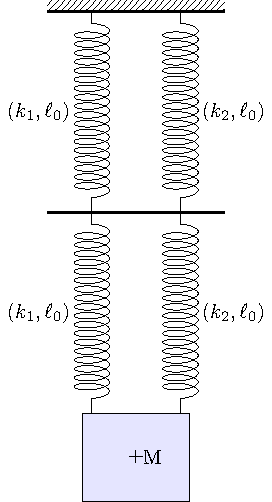
\includegraphics[width=\linewidth]{assemblage_complexe}
			\captionof{figure}{Assemblage complexe.}
			\label{fig:assem_cplx}
		\end{center}
	\end{minipage}
}

\end{document}
